\subsection{Proposal result}

To evaluate RUBY, we conducted the same experiment with other four
metrics to show the correlation of RUBY with semantic scores on two
model mppSMT and lpSMT. RUBY's efficiency was tested on a large number
of methods translated by those models.

\begin{figure}[t]
\caption{RUBY vs Semantic (lpSMT)}
\centering
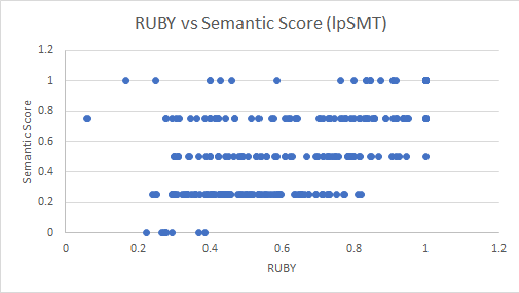
\includegraphics{img/rubyvssem_lpSMT.png}
\label{fig:RubySemlpSMT}
\end{figure}

\begin{figure}[t]
\caption{RUBY vs Semantic (mppSMT)}
\centering
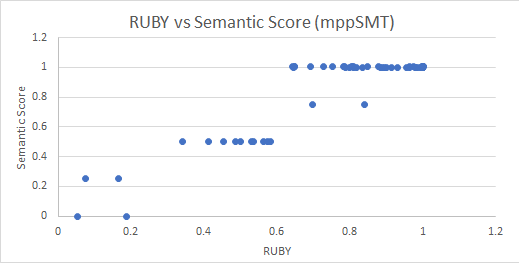
\includegraphics{img/rubyvssem_mppSMT.png}
\label{fig:RubySemMppSMT}
\end{figure}

Figures~\ref{fig:RubySemlpSMT} and~\ref{fig:RubySemMppSMT} show the
scatter plots between RUBY and Semantic scores on two models mppSMT
and lpSMT, respectively. As can be seen from the scatter plot for
lpSMT (Figure~\ref{fig:RubySemlpSMT}), there is a moderately strong,
positive, linear association between the two variables with a few
outliers.  Beside, the scatter plot for mppSMT
(Figure~\ref{fig:RubySemMppSMT}) shows a strong, positive, linear
association between RUBY and Semantic score. There are no outliers in
the data. This is the indication that the result is consistent.

In general, RUBY has high correlation with Semantic scores. As our
experiment result, the correlation coefficient between RUBY and
semantic score for model mppSMT is \textbf{0.862} and for the model
lpMSMP is \textbf{0.836}. In statistics, these values indicate a
strong uphill linear relationship between two quantitative
metrics. That means one metric could be predicted by the other with
high confidence. For example, an increase of 0.5, {\model} score can
be interpreted as an increase of 0.4 in term of Semantic score. Based
on that information, developers can tune the system in an incremental
manner.


%Specifically, a correlation of +0.8 implies that when 	

Although RUBY has a strong correlation coefficient, it is still lower
than GVED scores shown in Section~\ref{sec:alternatives} due to the
fact that only a subset of the dataset is applicable. While GVED is
only computed with the migrated code with sufficient semantic
information, RUBY does not depend on the code, even we can not parse
PDGs and ASTs. This implies that there exist a RUBY score for any
given code. On the other hand, in comparison with TREED, SED
and BLEU, RUBY always outperforms the other three metrics.
	    
  			
